\chapter{Architecture \& Concepts}

\begin{figure}[ht]
    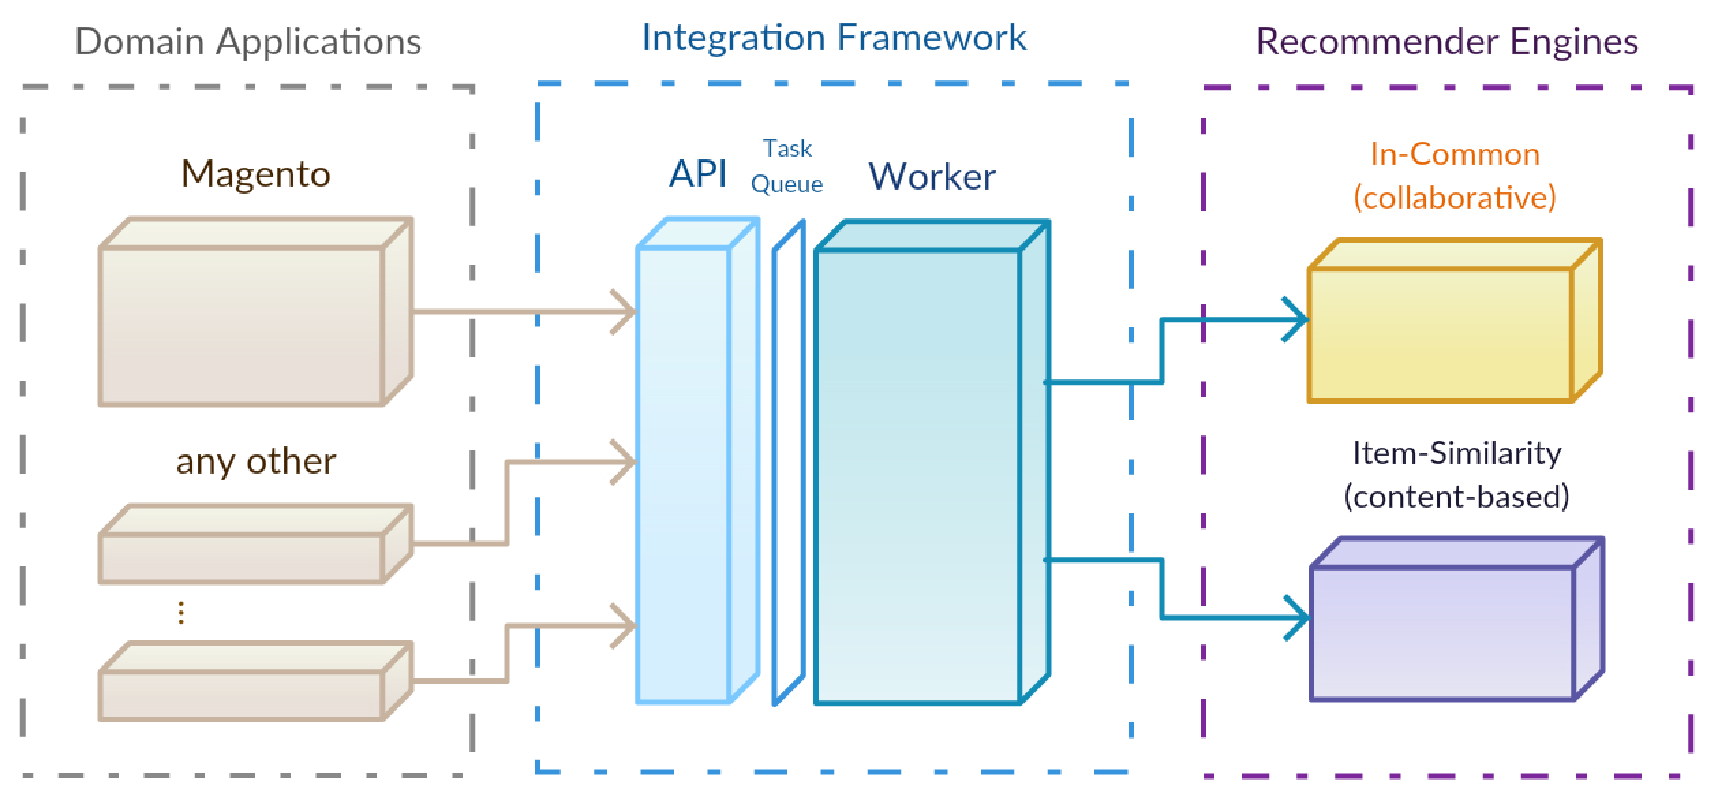
\includegraphics[width=\textwidth,center]{architecture/overview.pdf}
    \caption{Architectural Overview (Diagram)}
    \label{fig:architecture-overview}
\end{figure}

This chapter introduces essential concepts and discusses the architecture of the solution. Figure \ref{fig:architecture-overview} gives an overview of that architecture.

\section{Concepts}

In order to comprehend the architecture entirely, this section explains some essential concepts and terminology used in this project. Some terms are commonly used while others are specifically introduced in this project.

\begin{description}

\item[\textnormal{The} framework] or \textbf{integration framework} refers to the middleware implemented in the scope of this project.

\item[\textnormal{A} domain application] is an existing application primarily developed for a specific organisation or use-case, secondarily planning to make use of recommendations and integrate recommender engines. The definition highlights the fact that these systems are usually built on extensive domain knowledge. A typical application is e.g. in e-commerce which is demoed in this project.

\item[\textnormal{A} recommender engine] or \textbf{engine} is a system which suggests useful items to a user. A user is typically assisted in their search process to find the right items. Recommender engines are able to personalise this process so that they try to suggest only items relevant for the given user.

\item[\textnormal{A} recommendation request] is a query for recommendations and is processed by recommender engines via the framework. The response to a recommendation request is a \textbf{recommendation} -- a bespoke collection of items computed by the recommender engine.

\item[\textnormal{An} engine adapter] is a client software located in the framework and interacting with a recommender engine. Every engine to be used in the framework requires an adapter. The only two requirements are that they implement a method called \texttt{recommend} to perform the recommendation request and handlers for events a recommender has subscribed to.

\item[\textnormal{A} hybrid engine adapter] is a special engine adapter utilising two or more regular recommenders which are called \textbf{components}. In contrast to regular engine adapters, hybrid adapters do not provide handlers for event subscriptions.

\item[\textnormal{A} recommender] is a concrete use-case of a recommender engine and is configured in the framework. Beside the recommender engine, the configuration specifies events it subscribes to and a taxonomy. To give an example, \texttt{common_products_viewed} and \texttt{common_products_whitelisted} are separate recommenders but rely on the \emph{In-Common} engine. Similarly, a \textbf{hybrid recommender} is a use-case utilising a hybrid engine adapter. To put it in another way, recommenders are to engine adapters what objects are to classes.

\item[\textnormal{An} event] relates to any change or information recommenders need to be notified about. For collaborative recommenders these are usually user behaviour such as \emph{``customer viewed product''} or \emph{``user favourited movie''}. Content-based recommenders on the other hand would usually like to be notified about data changes such as items added, updated or removed. Events have an alphanumeric subject as well as a payload. Originally, it was proposed to have a separate \emph{master data} concept as well. It was dropped in favour of incorporating it into the event concept due to the fact that even master data changes are triggered by some kind of event such as creation and removal.

\item[\textnormal{A} taxonomy] is a data contract and mapping concept between domain and recommender engine terminologies as those are unknown to each other. It consists of \textbf{taxons} which define a map for a single term. The taxonomy describes the data fields the recommender expects from the domain application. It can also inherit from another taxonomy. Before the framework passes a data payload to a recommender engine, the data goes through the mapping process first.

\end{description}

\section{Domain Applications}
\label{architecture-domain-applications}

Section \ref{intro-bg-problems} already introduced domain applications and their problems caused by tightly coupling them with recommender engines. The technology stack is mostly tailored to the requirements of those systems and may not be the first choice for recommendation requirements. A solution is therefore to develop these requirements as a separate system, which is then integrated into the domain application. As explained in the introduction, this project is about developing such an integration framework to support this. Figure \ref{fig:architecture-overview} also shows that this project supports the integration of as many domain applications as required in a single framework installation.

Regarding knowledge, the proposed solution abstracts the internals of both domain application and recommender engines. In order for the domain application to do the integration, knowledge about the internals of recommender engines is not required. For this reason, the emphasis of the integration on the domain application side lies in the extraction of data of interest for recommendations. Furthermore, the terminology in this data can remain as it is.

\section{Recommender Engines}
\label{architecture-recommender-engines}

As was mentioned in the previous section, the technology stack of domain applications may not be the best fit for recommendation requirements and that a framework was developed to separate them. Originally, it was proposed to implement recommender engines against a uniform database natively within this framework. Yet while working on the project, it became obvious that the same technological fitness concern applied to the framework as well; in the sense that the technology stack of the framework may not be the best suited for recommender engines. Furthermore, the best suitable technology stack may differ substantially among recommender engines themselves.

Therefore it was decided to design recommenders as individual engines which allow the utilisation of not only the most suitable technology stack such as database management systems and programming languages but also existing, third-party recommender engines e.g. \emph{LensKit} or \emph{Apache Mahout}.

\section{Integration Framework}
\label{architecture-integration-framework}

\begin{figure}[ht]
    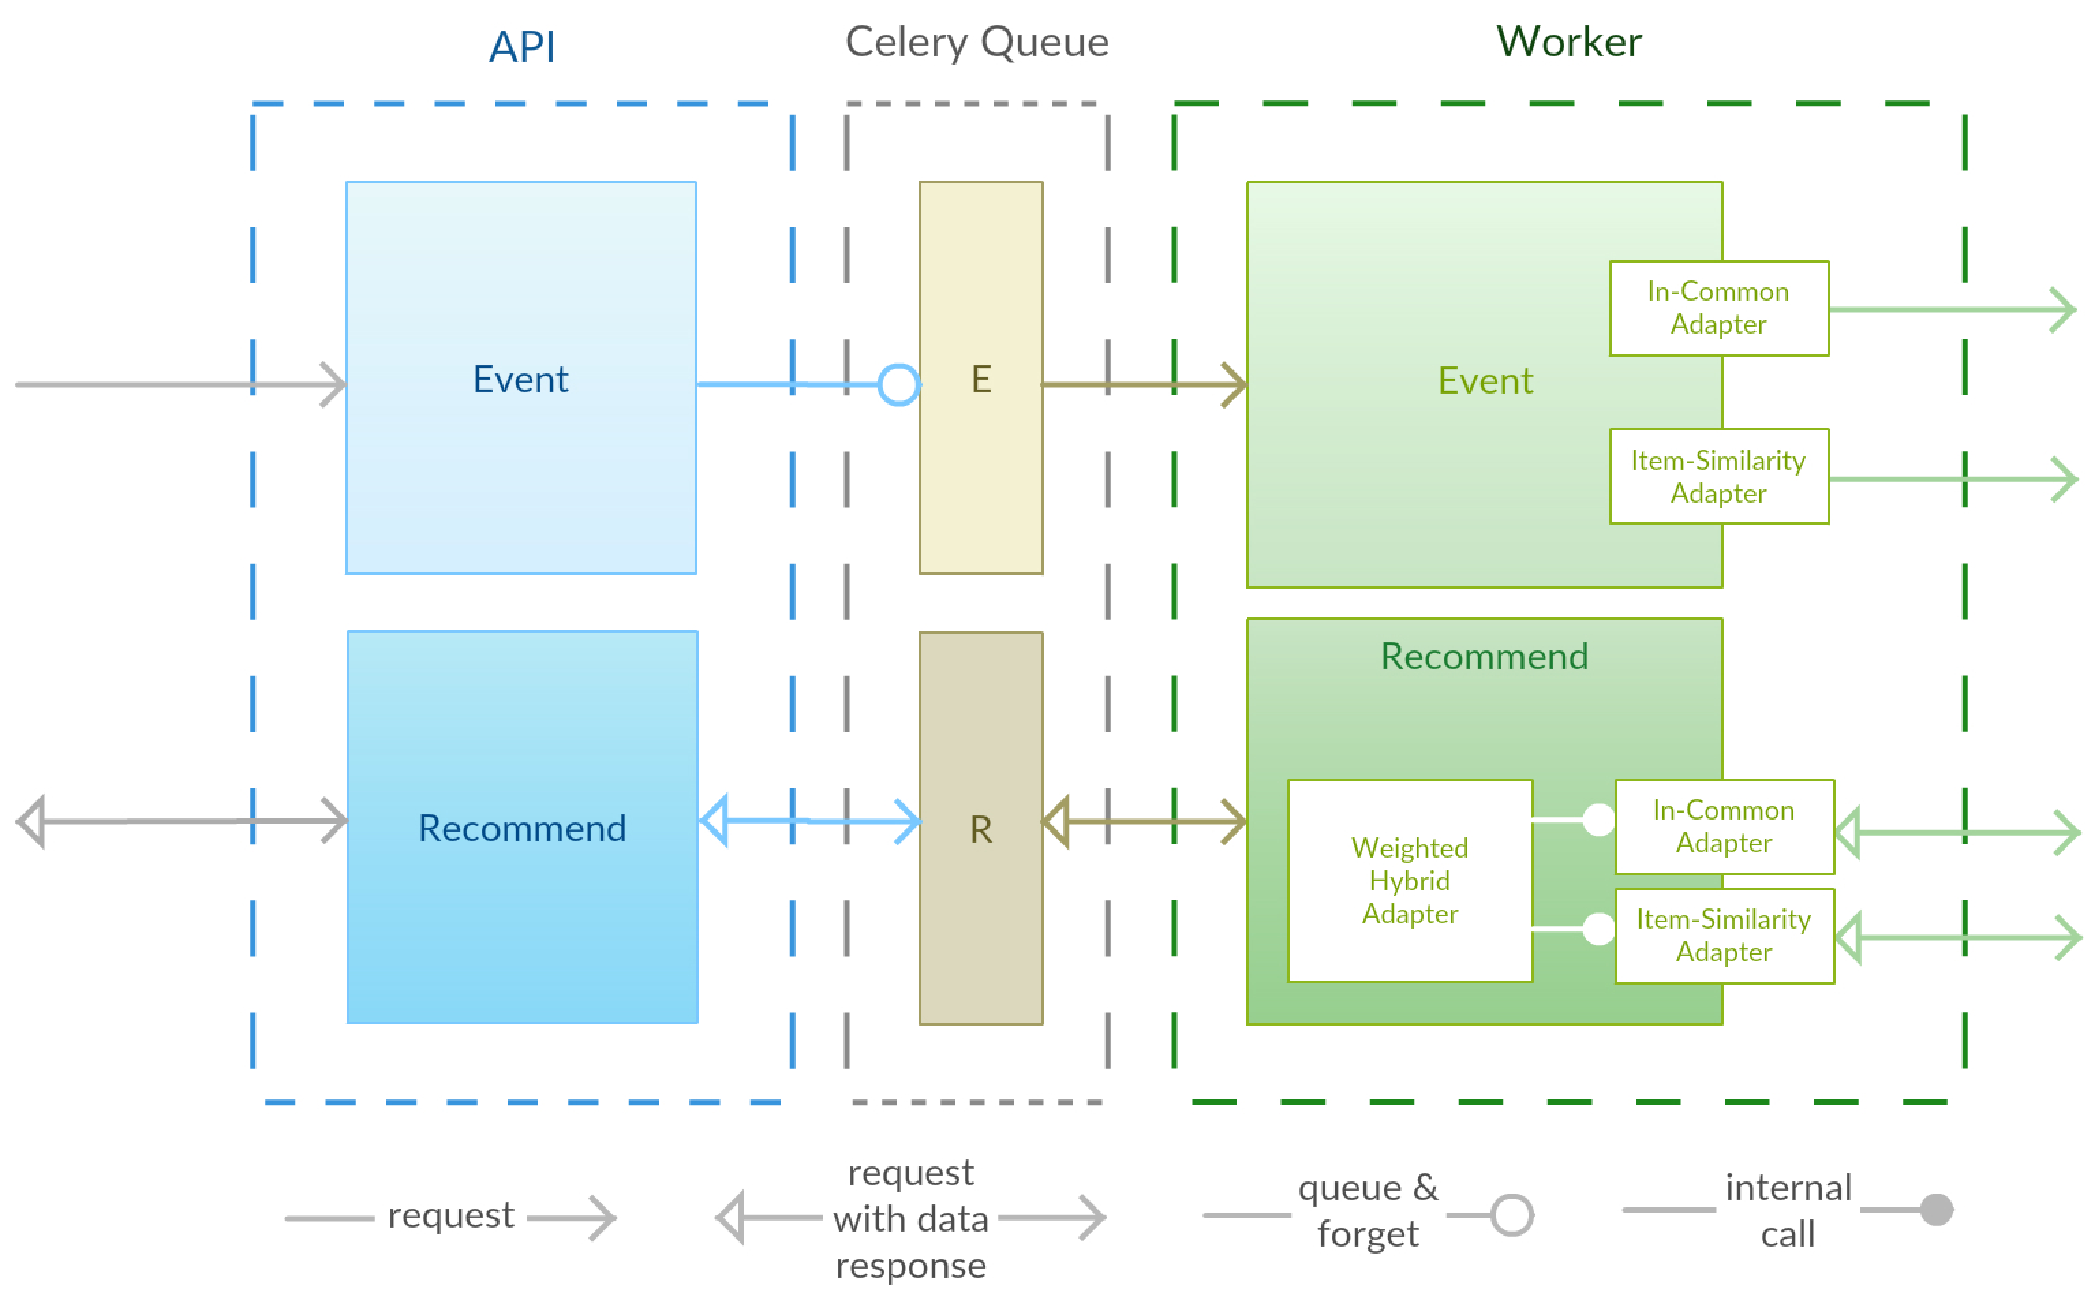
\includegraphics[width=\textwidth,center]{architecture/framework.pdf}
    \caption{Framework Design (Diagram)}
    \label{fig:architecture-framework}
\end{figure}

In the present report, framework relates to an integration tool to glue domain applications and recommender engines in a way which is \emph{multi-purpose}, \emph{easy to integrate}, \emph{encapsulated}, \emph{reusable} and \emph{technologically unbiased}. Since it is operating between two systems and not holding any actual logic, it can also be classified as a \emph{middleware}.

Figure \ref{fig:architecture-framework} shows a detailed diagram of the framework and makes two characteristics immediately visible: First, \emph{Event} and \emph{Recommend} are distinguished throughout the design of the framework. This reflects the \emph{service-oriented architecture (SOA)} as discussed in the project proposal. SOA suggests expressing features as services. Second, the framework is horizontally separated into layers which reflects the \emph{multi-layered} or \emph{multi-tier architecture} from the proposal. However, the project proposal suggested four layers: \emph{interface}, \emph{configuration}, \emph{recommendation} and \emph{persistence}. The final solution differs slightly. The API covers the interface layer whereas the configuration layer is more or less the workers. The layers recommendation and persistence are now regarded by the individual recommender engines.

\subsection{API}

The \emph{application programming interface (API)} is the endpoint (\emph{server}) for domain applications (\emph{client}) to interact with the framework. It is the only subsystem of the framework, which is exposed to other systems (also depends on the network configuration). The API adopts the architectural style \emph{representational state transfer (REST)} -- and is thus \emph{RESTful} -- via the \emph{hypertext transfer protocol (HTTP)} which is one of the fundamental protocols of the Internet and World Wide Web. Resources and actions compose REST APIs. Resources are uniquely referenced with \emph{uniform resource locators (URLs)}. Actions specify the operation to happen on a resource which is described by \emph{HTTP vocabularies} amongst others \emph{GET} and \emph{POST}. Both URLs and HTTP vocabularies are basics of the Internet and are almost self-explanatory which results in more compact documentation \cite{fielding00}.

An essential property of REST is \emph{statelessness} and says that the server should not remember any state of the client. \citet{fielding00} further states that statelessness improves visibility, reliability and scalability. Visibility is improved by the fact that a request by a client has all information necessary to understand. Reliability is improved because a request is not affecting others and makes recovery of partial failures easier. Finally, better scalability can be observed as the server does not need to manage state data between requests.

The framework has two APIs: \texttt{Event} handles event notifications as \emph{POST} requests whereas \texttt{Recommend} handles recommendation queries as \emph{GET} requests. As far as the framework is concerned, its API bears no business logic at all and hands requests over to the workers via a task queue which is going to be covered in the next section.

\subsection{Task Queue}

A \emph{task queue} is a software system for managing tasks using \emph{message queues}. The latter store messages sent by a publisher and enable one or more consumers to read messages in \emph{first in, first out (FIFO)} order. Amongst other benefits, message queues allow communication between independent systems and can help scaling by distributing messages to more than one consumer. Similarly, task queue systems offer a mechanism to run tasks on independent systems and distribute them to a group of processes. It hides the internals such as serialisation of task contexts as well as handling errors and responses.

Figure \ref{fig:architecture-framework} illustrates the task queues \emph{Event} and \emph{Recommend}. Albeit task queue systems can manage different tasks via a single queue, it was decided to use designated queues to give prioritisation of recommendations over event tasks. In practice, it means that a real-time recommendation query for a website user has to be processed sooner than eventual events. The Event API runs tasks asynchronously and does not wait for a result (\emph{queue \& forget}) whereas the Recommend API waits for the result -- namely a list of recommended items.

\subsection{Workers}

\emph{Workers} are background processes and consume tasks from aforementioned task queues. Unlike the API, workers are doing the actual processing. Similar to API and queues, they are also divided into \emph{Event} and \emph{Recommend} workers. Workers are designed to scale horizontally by running more instances.